\chapter{Development}

This chapter describes the development of my application, SpiDB, from September 2015 to March 2016, involving planning, testing and implemention. The SpiNNaker project is open-source and so is my application, which can be found on the url \textit{https://github.com/SpiNNakerManchester/SpiNNakerGraphFrontEnd}.
By being part of the SpiNNaker team in Manchester, I was directly exposed to the ongoing research, frequently receiving feedback on my work. The collaboration was effectively bi-directional, as I was able to constantly find, evaluate and fix inconsistencies and bugs in the API not known to the team.

\section{Testing and Debugging}

\section{Bugs}
I have been one of the few users of a large amount of the SpiNNaker API, currently under contruction. This means some of it has not been fully tested, resulting in strange behaviour at times, making debugging of my own application difficult.

blah blah test usability
particularly

Although not being directly part of the project, 

MENTORING

\begin{itemize}
\item \textbf{Duplicate packets:} when multiple distinct SDP packets were sent from different sources to the same destination, strangely the receiving core would read the same packet duplicated a number of times. This behaviour was unexpected, so upon extensive testing and collaboration from the team, I was able to point the issue to a running processor binary named \textit{reinjector} and resolve the issue. 

\item \textbf{Data Specification Error:} when uploading binaries to the board, sometimes cores would crash with the SWERR state. After giving the team detailed feedback on the issue, this was found to be caused by the SpiNNaker Data Specification framework, which handles allocation of data in shared RAM.

\item algorithms

\end{itemize}

From planning, design, testing, development, code review, etc. presentation of results to members of the Spinnaker team

It outlines also my approach and design choices with their advantages/disadvantages with the hardware and specification. (eg. no acknowledgements)
Approval from members of the SpiNNaker team.

Strengths and weaknesses (limitations) of spinnaker
...
Thomas, etc.
tutoring! kind of did it really


...upload different programs to run on each core.
Thus each chip contains the following instances: 

test-first development

what order I did things, etc.
learning curve
fixing bugs, helping spinnaker team etc.
Bizantine protocol

\section{Planning and Design}
In September I participated on the XXXth spinnaker workshop...
API, etc.

key-value then relational

\section{Implementation}

\section{Evaluation}

\subsection{SpiNNaker Communication fabric}

XXXX should this be on the introduction???
event driven

The SpiNNaker API allows the utilisation of 4 different communication protocols between cores in the system. These packets trigger prioratised interrupts on the receiver, as it is an event driven architecture. These can be used to spread work load and transmit information initially private to a core.
It is worth noting that \textbf{none of these protocols guarantee successful delivery of data} and this effect is worsen if there is large traffic in the communication fabric. This means sending a large amount of packets symultaneously will result on packet drops.

\begin{itemize}
\item \textbf{Multicast (MC)}
The MC protocol, originally designed to simulate neural spikes, predicts a sigle source core casting a packet to multiple destinations. The packet contains only a 32 bit routing key, used by an external process to carry out the delivery, and an optional 32 bit payload, both provided at the source.

router.. routing table
\item \textbf{Point to Point (P2P)}
XXX
On top of the P2P layer, the SpiNNaker Datagram Protocol (SDP) was developed (build/written?) to allow larger transfers of data, of up to 280 (?) bytes, to reduce queueing on receival... (find the paper...)
%https://spinnaker.cs.man.ac.uk/tiki-download_wiki_attachment.php?attId=16

Using SDP, the SpiNNaker API XXX a User Datagram Protocol (UDP), allowing a two-way communication over IP addresses with the host machine. This allows uploading binaries and communicating back and forth with the hardware.

unreliability....
unreliable spikes (see that guy's paper...)

\item \textbf{Nearest-neighbour (NN)}
\item \textbf{Fixed-route (FR)}
\end{itemize}

[spinnaker datasheet page 30]

-mention DTCM only 64kb (so preferred to use SDRAM)
-look at your logbook for query plan stuff (at the start)
-debugging with ybug. testing with unit tests
-supported operations
-host is stateless
-tested on real data?

Each processor node on SpiNNaker includes a communication controller which is responsible for generating and receiving packets to and from the communication network.
The SpiNNaker architecture offers a range of...
all of which are unreliable!!

packet formats:


A tree structure composed of \textit{root}, \textit{branch} and \textit{leaf} nodes. The tree structure presented by my database management system allows a divide and conquer approach to the database query plan. This means when queries are issued by the \textit{host}[definition] and received at the \textit{root}, they are broken down and forwarded for parallel processing through \textit{branch} and \textit{leaf} nodes. eg. COUNT, MAX, MIN, AVG, SUM

problems:
sending a large amount of packets with little or no delay xx kills xx the core. sending more than about 4 packets symultaneously at a destination results on a very high packet loss (2/3 of SDP packets get dropped).


solutions:...
delays
tree structure
no acknowledgement


This approach has the following advantages (compared to a flat structure)
-a core will only ever receive packets from up to 4 other cores symultaneously (branch: 4, root: 1, leaf: 1), which is the limit of reliability.
-aggregation of results can be done in iterations/stages

disadvantage:
-less leaf nodes (which do the actual work)

LIMITATION:
no global timer, the maximum we can do is a timer for each chip (collection of 18 cores)
reliability

COMPLEXITY

limitation:
-single point of failure for each board(mention that it is already like that. no way to avoid).
-SDRAM bandwidth

scalability

message id and all other fields, etc.

\begin{itemize}
\item 1x \textit{sark} - monitor process provided by the API to handle low level SpiNNaker operating system functions
\item 1x \textit{reinjector} - utility process provided by the API to allow automatic re-propagation of dropped multicast packets
\item 1x \textit{root} - central node which handles direct communication with host machine via UDP and redirects incomming queries to respective cores. 
\item 3x \textit{branch} - intermediate node which aggregates queries from 4 leaf nodes and communicates back to host via UDP (why 4? because 4 sdp channels?). 
\item 12x \textit{leaf} - receives insert/retrieve queries from the root, processes the request and then returns result to branch node
\end{itemize}
why branches, etc?

\begin{figure}
\begin{center}
	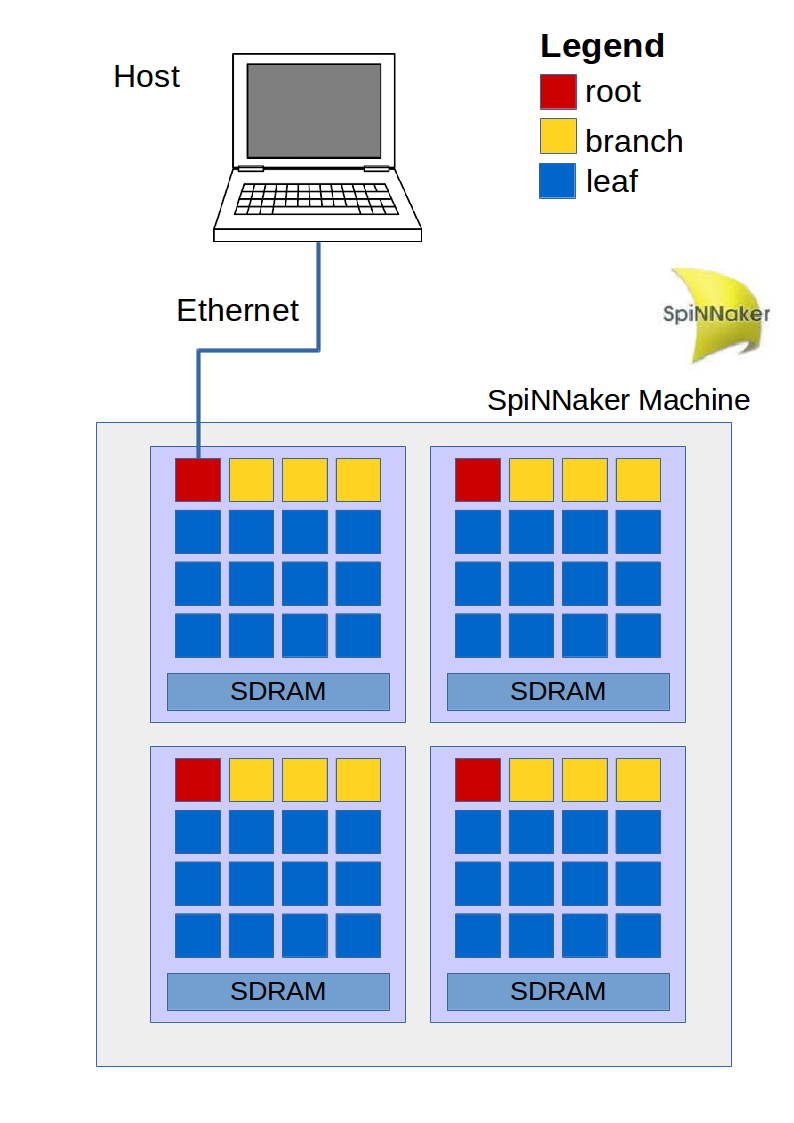
\includegraphics[width=0.8\textwidth, natwidth=794, natheight=1123]{images/spiDB_architecture.png}
\end{center}
\caption{SpiDB Architecture}
%\label{fig:die-plot}
\end{figure}


\subsection{PUT}

Syntax:\\
\noindent
 {\large\textbf{put} \textit{(int|string)}:key \textit{(int|string)}:value} \\\\

The \textbf{put} operation is the main way of inserting data onto the SpiDB distributed database. 
Upon completion, such operation will store the specified key, mapping to its value, on the memory of an arbitrary chip in the Spinnaker board (as chosen by the root core). This operation expects an acknowledgement from the core which stored the entry.\\\\

\noindent
 Example usage:\\
 \begin{lstlisting}
 put "hello" "world"
 put 123 "foo"
 put "life" 42
 put 1 2
 \end{lstlisting}
\noindent 
 Complexity: linear to the size of the input key-value, constant to database size.\\\\
 
Steps:
\begin{enumerate}
\item User issues query of format \textit{put "key" "value"} on host machine
\item Query and metadata are converted into a byte array with the following format, transferred over UDP socket to the board

\lstinputlisting[language=C]{code/putQuery.c}

Where \textit{info} contains the metadata regarding the entry to be stored. It is composed of 32 bits, ...
[bits bits bits, etc]

how is it actually stored??? !!?!! say it and mention word alignment

\item Packet transfer triggers interrupt on \textit{root} core, which selects a \textit{leaf} core to store the data entry (hash or Round Robin...?) and communicates to it via SDP
\item \textit{leaf} triggers an interrupt and stores key-value entry into its dedicated region of SDRAM
\item \textit{leaf} sends an acknowledgement message over UDP back to host
\end{enumerate}

\subsection{PULL}

 Syntax:
 \noindent
 {\large\textbf{pull} \textit{(int|string)}:key}\\\\
 
The \textbf{pull} operation is the main way of retrieving data from the SpiDB distributed database.
When the operation is issued, the SpiNNaker cores will be coordinated to search for the given key and, if found, the value mapped by it will be returned to host. If the key does not exist, no reply is given, resulting on a timeout on the host (reason for this...). This means 
-disadvantage: expensive if not found
-advantage: less packet drops as less internal communication traffic
 
\noindent
 Example usage:\\
 \begin{lstlisting}
 pull "hello"
 pull 123
 \end{lstlisting}
 Assuming successful execution of the put commands above, such pulls would return "world" and "foo" respectively.\\\\
 Complexity: linear to the size of the input, linear to database size.\\\\

\begin{enumerate}
\item User issues query of format \textit{pull "key"} on host machine
\item Query and metadata are converted into a byte array, transferred over UDP socket to board
\item Packet transfer triggers interrupt on \textit{root} core, which issues a \textit{multicast} packet to all \textit{leaf} nodes requesting them to search for occurences of "key"
\item \textit{leaf} triggers an interrupt
\begin{itemize}
\item If a \textit{leaf} node identifies "key" by scanning linearly through SDRAM, it responds to host (branch...?) with mapped value
\item Else no response is sent, yielding timeout on host (reason for this!!!...?)
\end{itemize}
\end{enumerate}

how the data is actually stored?

SQL:
column based?

bandwidth (max) vs throughput (actual)


identifies
flow control of:
put
pull
etc.

Upon completion of the project, 

 \newpage
\noindent 
  {\large\textbf{CREATE TABLE} \textit{(string)}:tableName(\\
  	\textit{(string)}:column1 integer|varchar(\textit{int}),\\
  	\textit{(string)}:column2 integer|varchar(\textit{int}),\\
  	...\\
  	);}\\\\
\noindent
  Reserves memory space for an SQL table and stores its metadata. This operation expects an acknowledgement.\\\\
   Complexity: linear to the size of the input, constant to database size.\\\\
 \noindent
  {\large\textbf{INSERT INTO} \textit{(string)}:tableName(\textit{(string)}:column1,\textit{(string)}:column2,...)\\
  \textbf{VALUES}(\textit{(int|string)}:value1,\textit{(int|string)}:value2,...);}\\\\
\noindent
  Inserts specified values on the given table's memory space at an arbitrary chip. This operation expects an acknowledgement.\\\\
\noindent
   Complexity: linear to the size of the input, constant to database size.\\\\
\noindent
  {\large\textbf{SELECT} *|\textit{(string)}:column1,\textit{(string)}:column2,...\\
  \textbf{FROM} \textit{(string)}:tableName\\
  \textbf{WHERE} \textit{(string)}:column|\textit{(int|string)}literal \\=|!=|\textless |\textless =|
  \textgreater | \textgreater = \textit{(string)}:column|\textit{(int|string)}literal;}\\\\
\noindent
  Retrieves a list of entries corresponding to the previously inserted values on given table which match the WHERE criteria. Matching results are streamed in until timeout is reached. If no value matches the criteria, the Spinnaker board will not respond.\\\\
\noindent
Complexity: linear to the size of the input, linear to database size.\\\\
  

\begin{figure}
\begin{center}
	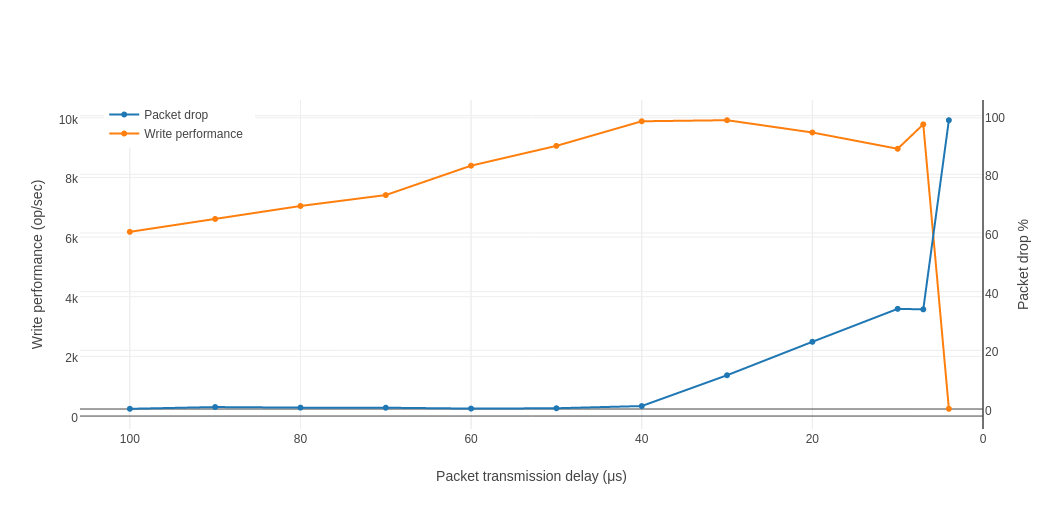
\includegraphics[width=1.4\textwidth, natwidth=1063, natheight=509]{images/transmission_delay.png}
\end{center}
\caption{Transmission delay plot}
\label{fig:die-plot}
\end{figure}

%\caption{Die plot of the SpiNNaker CMP}

done:
blocking vs non-blocking

future work...
cache (on DTCM)
aggregation
CGI server
self balancing when IDLE (ie. move data to cores with less data, if a table is about to get full, move data around it's SDRAM) --- user typing = a long time
million core machine
improve parser
allow longer queries in (more than 256 bytes)
additional operations eg. delete, update, etc,...
more reliability
ACID properties

\lstinputlisting[language=C, caption=SDP Packet Callback]{code/sdp_packet_callback.c}

callback priorities etc.

cannot possibly do more than that...
ARM968 at only 600MHz (I think)

response times. why are they so high sometimes?!?!
-first explain how we gather the time (operating system could be interrupting, sark, etc.)


hash vs naive
